%%%%%%%%%%%%%%%%%%%%%%%%%%%%%%%%%%%%%%%%%%%%%%%%%%%%%%%%%%%%%%%%%%%%%%%%%%%%%%%%
%%%%%%%%%%%%%%%%%%%%%%%%%%%%%%%%%%%%%%%%%%%%%%%%%%%%%%%%%%%%%%%%%%%%%%%%%%%%%%%%
\section{Percepção da métrica no samba}
\index{Musicalidade!Métrica no samba}
\label{sec:percepcaosamba1}

As músicas dos subgêneros do samba, as quais usamos para dançar, 
geralmente são escritas usando \hyperref[subsec:compassobinario]{\textbf{compassos binários}};
por este motivo a procura da métrica das músicas nesses subgêneros 
é mais simples, 
pois iniciamos a busca tendo a quase certeza do tipo do compasso, 
pelo que só precisaríamos \hyperref[subsec:perceberTF1]{\textbf{achar o tempo forte}} 
usando as indicações descritas na seção \ref{subsec:perceberTF1}.

Assim, para detetar o tempo forte e as \hyperref[sec:pos:Duracion]{\textbf{durações}} dos tempos nos compassos,
devemos ter em conta que quando escutamos uma música 
na qual é tipicamente dançado o samba, ou especificamente o samba de gafieira,
podemos distinguir que a união dos sons produzidos pelos instrumentos de percussão\footnote{Ou o
acompanhamento em geral.} 
geram um padrão de repetição muito particular, 
geralmente relacionado com as onomatopeias: ``tchic tchic tum'' ou ``tum tum''; 
em ambos  casos existe um  ``tum'' executado com maior 
\hyperref[sec:pos:Intensidade]{\textbf{intensidade}} (potencia sonora) e
que está sendo executado no tempo forte.
Se conseguimos detetar ou encaixar alguma destas duas onomatopeias na música,
então temos o problema resolvido, pois ambas ocupam exatamente dois tempos 
e dado que para conseguir encaixar as onomatopeias tivemos que reconhecer o tempo forte no ``tum'',
temos todos os elementos para descrever a métrica dos compassos na música.

\PRLsep{Analisando a música no samba}

A Figura \ref{fig:abc-caquarela} representa os compassos 18, 19 e 20 da  
composição musical ``Aquarela do Brasil'' escrita
por Ary Barroso em 1939 \cite{AquarelaDoBrasil}; 
a versão mostrada na figura teve arranjos por Irineu Krüger \cite{Irineu}.\\ 


\begin{figure}[ht]
\centering
\href{https://drive.google.com/file/d/1RcUcWJlukxaF7nmDTKDxUZDR8sLH9QpC/view?usp=sharing}{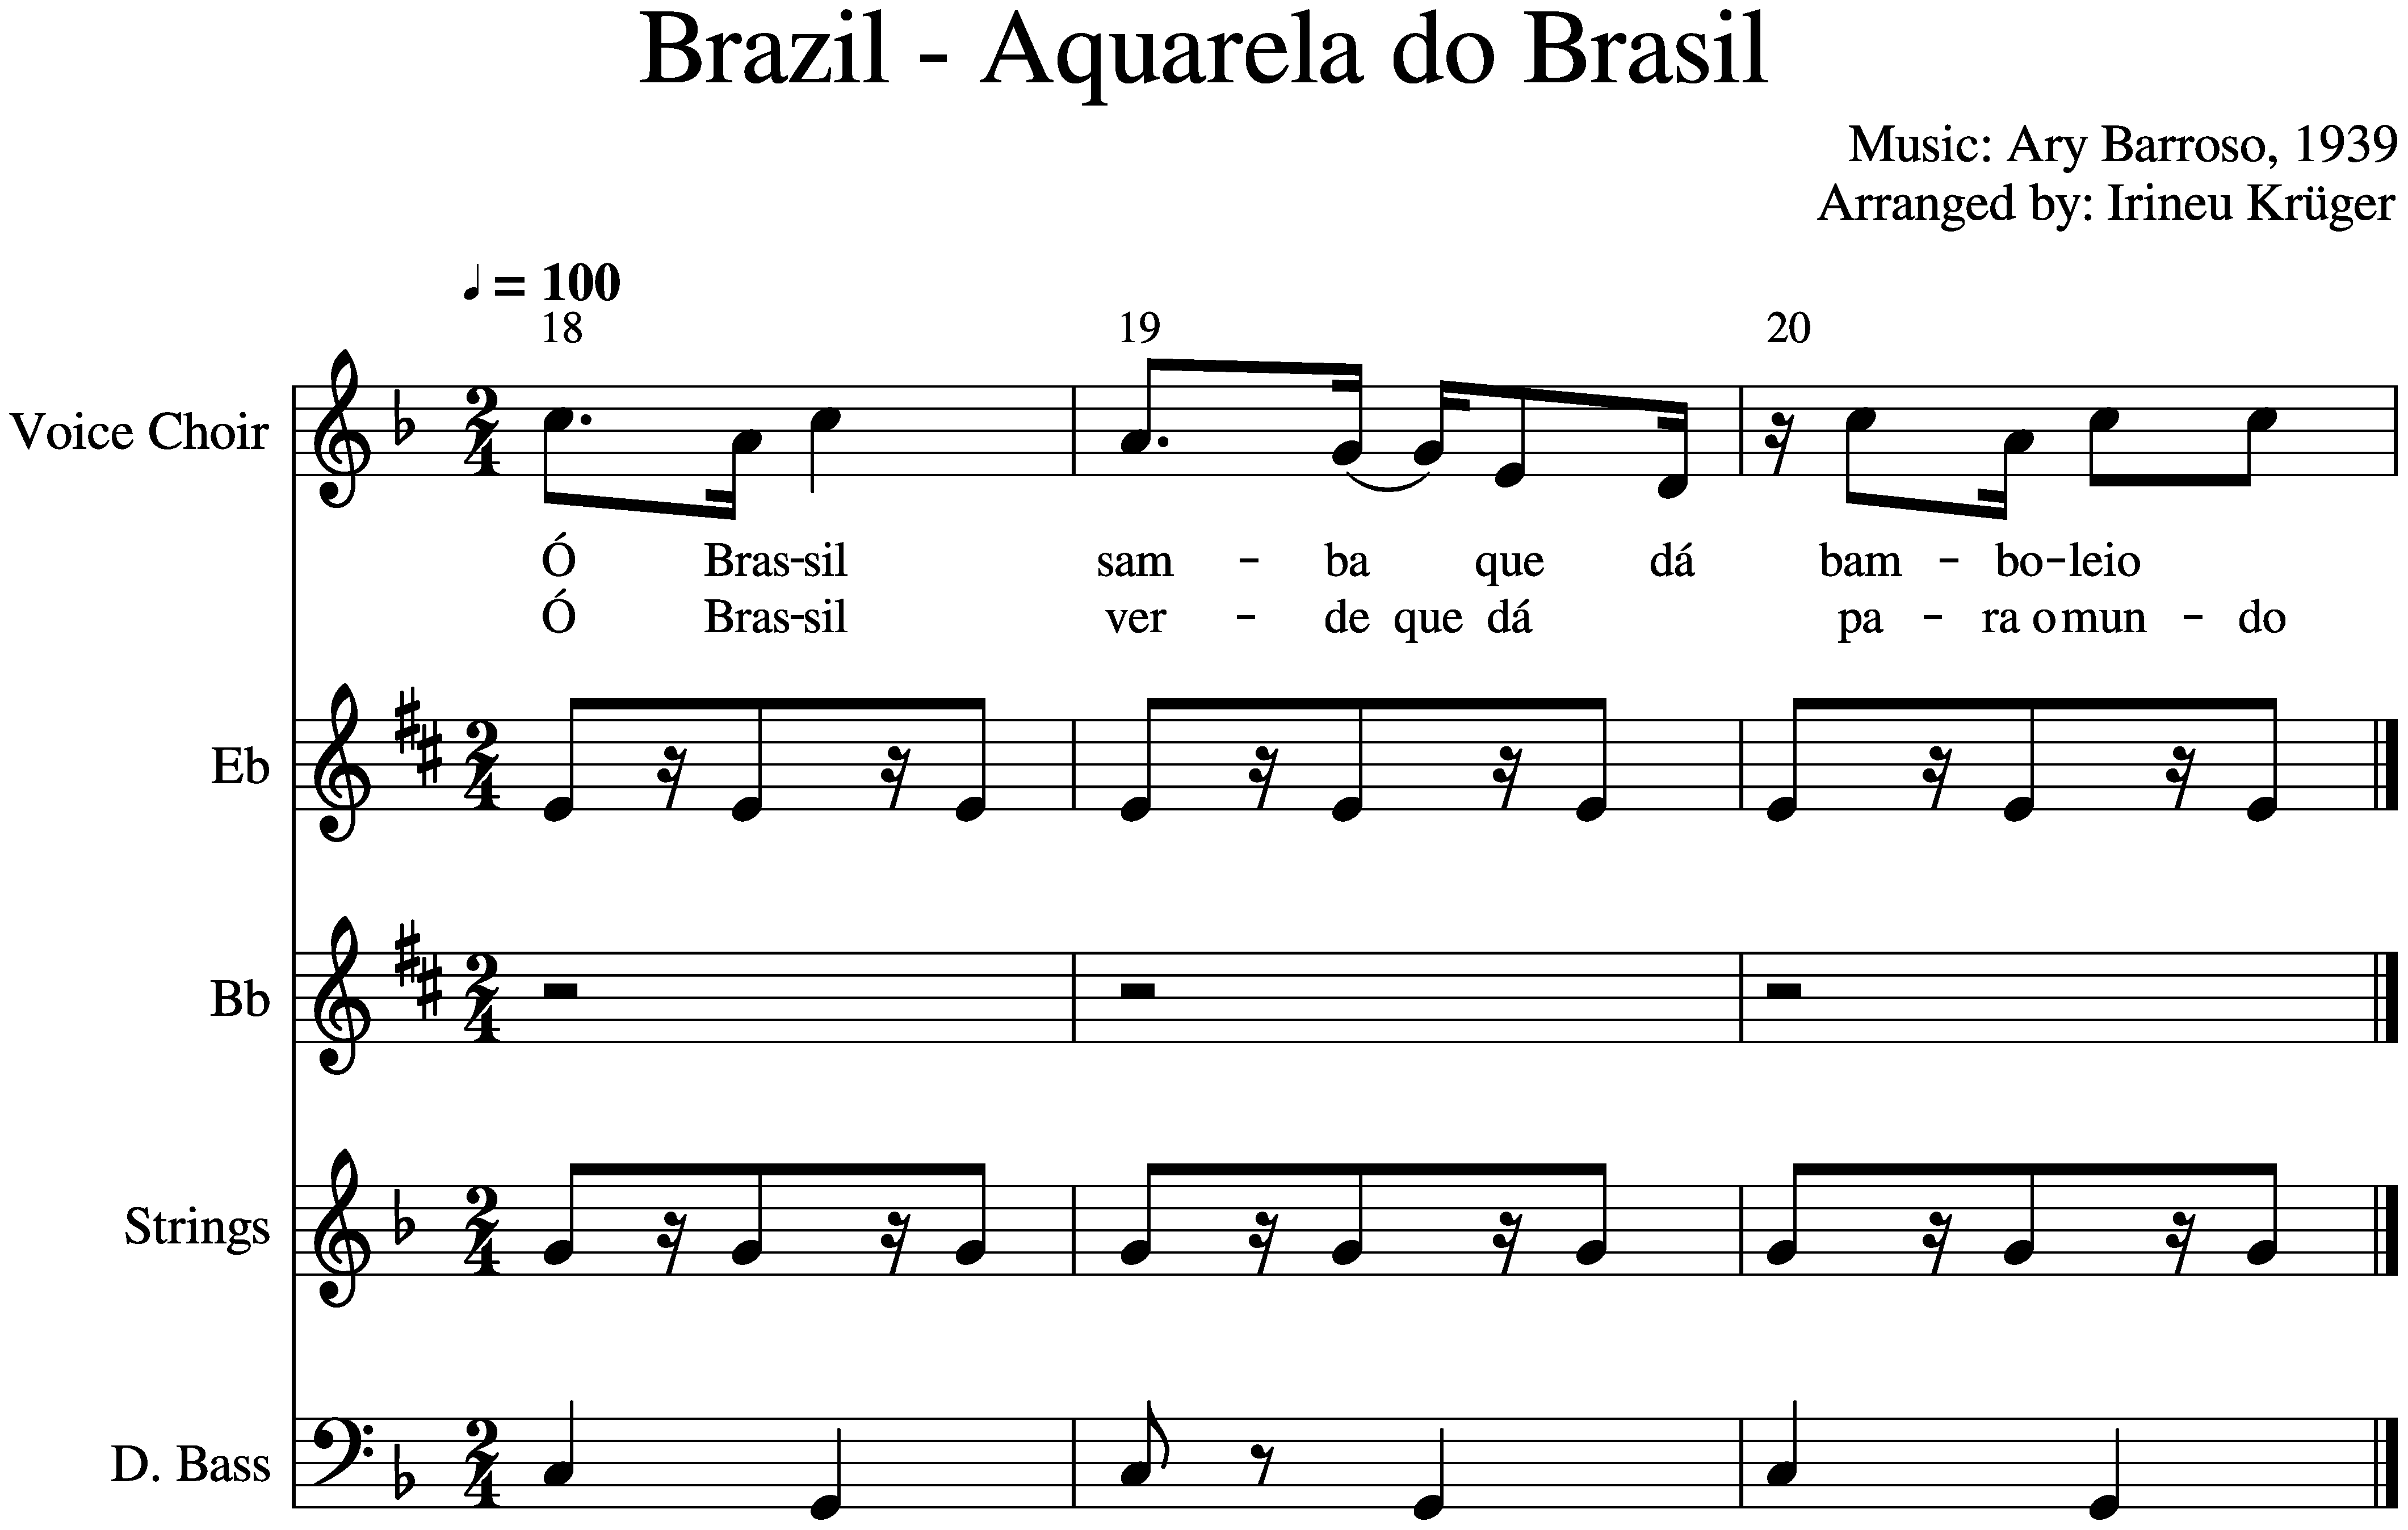
\includegraphics[width=0.99\textwidth]{chapters/cap-musicalidade-percepcion/abc-aquarela-1.eps}}
\begin{comment}
\begin{abc}[name=abc-caquarela]%,options={-O= -c -s 0.8}]
% abcm2ps aquarela.abc  -O aquarela.ps
% ps2epsi aquarela.ps aquarela.eps
%
X: 1 % start of header
T: Brazil - Aquarela do Brasil
C: Music: Ary Barroso, 1939
C: Arranged by: Irineu Krüger
K: Dm % scale: C major
Q:1/4=100
M: 2/4 % formula do compasso
%
V:1 clef=treble name="Voice Choir" sname="Voice Choir"
V:2 clef=treble name="Eb" sname="Eb"
V:3 clef=treble name="Bb" sname="Bb"
V:4 clef=treble name="Strings" sname="Strings"
V:5 clef=bass   name="D. Bass" sname=""D. Bass"
%
%
[V:1] "18" C'3/2A/2C'2  |"19" A3/2(G/2 G/2)E1D/2  |"20" z/2 C'1A/2 C'1C'1  |
w:    Ó Bras-sil        sam-ba_ que dá       bam-bo-leio_ 
w:    Ó Bras-sil        ver-de que dá_       pa-ra~o mun-do 
%
%
[V:2] [K:D] E1z/2E1z/2E1  | E1z/2E1z/2E1  | E1z/2E1z/2E1  |
%
%
[V:3] [K:D] z4  | z4  | z4  |
%
%
[V:4] [K:Dm] G1z/2G1z/2G1  | G1z/2G1z/2G1  | G1z/2G1z/2G1  |
%
%
[V:5] C,2 G,,2  | C,1 z1 G,,2  | C,2 G,,2  |
\end{abc}
\end{comment}
\caption{3 compassos da partitura da composição ``Aquarela do brasil''.}
\label{fig:abc-caquarela}
\end{figure}

Nesta versão, a música está escrita seguindo uma 
\hyperref[subsec:homofonica]{\textbf{textura homofônica}} com:
\begin{itemize}
\item \textbf{melodia principal:} 1 voz ou coro de voces (``Voice Choir'') e  
\item \textbf{acompanhamento:} 4 instrumentos (``Eb'',``Bb'',``Strings'' e ``D. Bass''), 
\end{itemize}
que usam uma 
formula de compasso $2/4$, de modo que se tem compassos
binários com tempos com uma \hyperref[sec:pos:Duracion]{\textbf{duração}} de uma semínima (\quarternote).


\begin{figure}[hb!]
\begin{elaboracion}{Jaime Arôxa e o ``tic tic tum''}
\index{Musicalidade!Tic tic tum}
\begin{wrapfigure}{r}{0.35\textwidth}
\centering
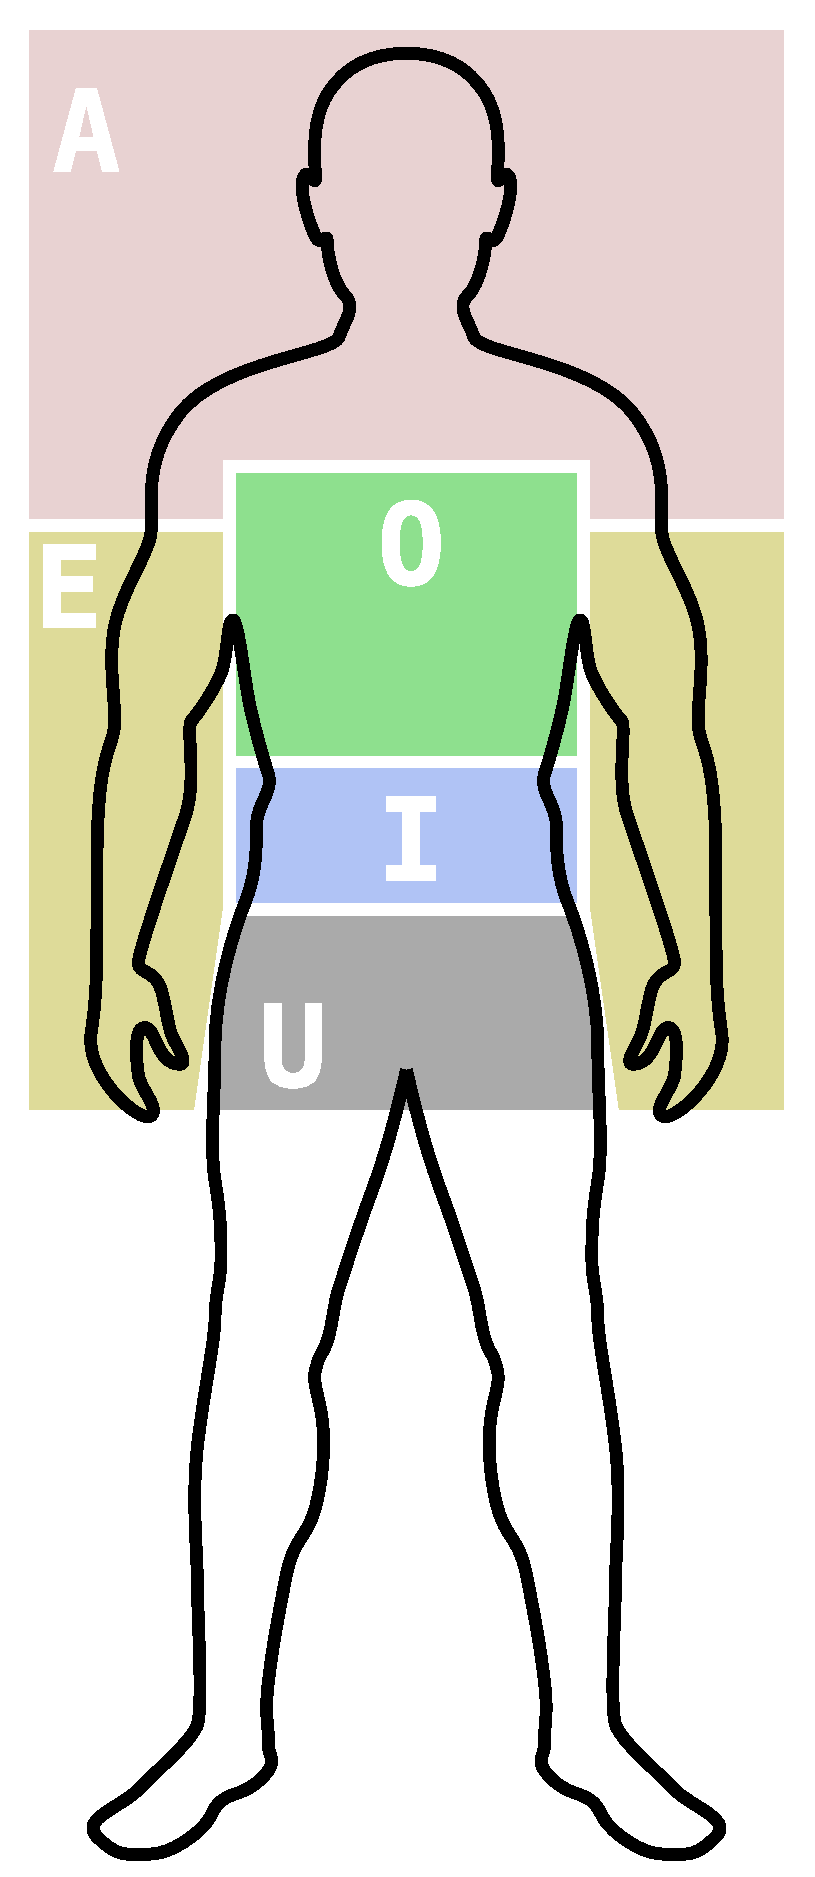
\includegraphics[width=0.33\textwidth]{chapters/cap-musicalidade-percepcion/aroxa-tic-tic-tum.eps}
\end{wrapfigure}
O renomeado professor de dança, coreografo e  dançarino, Jaime Arôxa \cite{JaimeAroxaSite},
numa de suas múltiplas contribuições ao ensino da dança de salão no Brasil,
criou ao redor do ano de 1991, 
o uso do ``tic tic tum''
\footnote{Popularmente também pode se achar o termo ``tchic tchic tum'' que tem só um sentido temporal, 
e não corporal como na didática proposta por Jaime.} 
para o ensino do ritmo nas aulas de samba de gafieira \cite{EntrevistaJaimeAroxa1};
numa tentativa de aproximar conceitos musicais a pessoas não iniciadas em música;
de modo que ele, na sua didática, não usava números e sim sons que eram fáceis de lembrar e interpretar.
Na sua proposta pedagógica, 
Jaime indica que cada parte do corpo pode estar atrelada a uma vogal.
\begin{description} 
\item[A:] Cabeça e ombros. 
\item[E:] Braços e mãos. 
\item[I:] Umbigo.
\item[O:] Embaixo dos ombros e o peito.
\item[U:] Bacia.
\end{description}
Assim, mecanicamente falando, o ``tic tic tum'' é ideal para o ensino do samba de gafieira
\footnote{Jaime ao redor do ano de 1991 criou o uso de ``tum e tum'' para bolero;
e em anos posteriores ``tum tum pá'' para o ensino de zouk.},
pois:
\begin{itemize} 
\item o ``tic'' está relacionado com uma contração do umbigo para deixar as pernas mais soltas;
\item o ``tum'' indica uma transferência total do peso do corpo pela ação da bacia;
\end{itemize}


Por outro lado, falando temporalmente, um ``tic tic tum'' descreve um ritmo com uma distribuição de tempos, 
no qual um ``tic'' dura a metade de tempo que um ``tum''. 
Uma forma de representar isto na notação musical pode ser vista na seguinte pauta.\\

\centering
\href{https://drive.google.com/file/d/1CZaAP5lPzVX7oTT5EMpIKN-XbOUYUt3Y/view?usp=sharing}{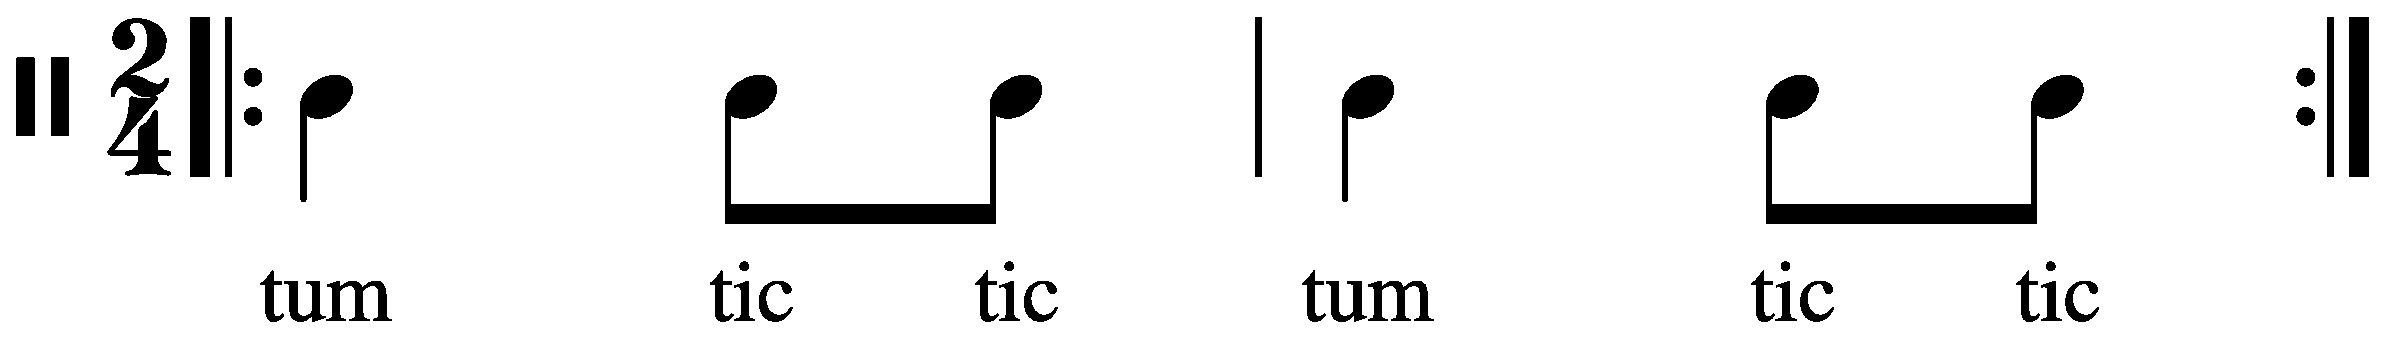
\includegraphics[width=0.7\textwidth]{chapters/cap-musicalidade-percepcion/abc-tictictumaroxa-1.eps}}
\begin{comment}
\begin{abc}[name=abc-tictictumaroxa,width=0.60\linewidth]
X: 1 % start of header
K: C stafflines=0 % scale: C major
M: 2/4 %meter - compasso
V:1 clef=perc stem=up %name="Pauta com clave de fá"   sname="Pauta com clave de fá"
[V:1] |:B2 B1 B1 | B2 B1 B1:|
w: tum tic tic tum tic tic
\end{abc}
\end{comment}
\end{elaboracion}
\end{figure}


\subsection{Percepção do: tchic-tchic tum}

Analisando o fragmento de partitura da Figura \ref{fig:abc-caquarela} e escutando a música produzida, 
podemos perceber que os instrumentos executados em conjunto geram um sonido identificável
com a onomatopeia ``tchic tchic tum'', com uma duração de dois tempos.
Assim, o inicio de cada compasso coincide com o ``tum''; 
sendo que este é o momento em que a maioria dos instrumentos produzem um sonido, 
de modo que a sensação para o ouvinte é de uma potencia sonora maior. 
Cada instrumento prolongará seu sonido de forma diferente; 
porém,  podemos dizer que: o ``tum'' ocupa $1$ tempo (\quarternote), 
e que o sonido de um ``tchic'' ocupa médio tempo (0.5\quarternote),
sendo que o primeiro ``tchic'' é executado no tempo fraco de ``D. Bass'', 
e o segundo ``tchic'' solapa e obscurece ao  primeiro, 
que é executado na parte fraca do tempo fraco de ``Strings'' ou ``Eb'';
conseguindo assim criar a ilusão da onomatopeia ``tchic tchic tum'', 
com ``tchic''s de médio tempo; de modo que:
\begin{equation}
tchic + tchic = tum ~~ \Longleftrightarrow ~~ tchic = \frac{tum}{2}.
\end{equation}
 
Por outro lado, se a percepção do ouvinte é mais
aguçada, poderá escutar a onomatopeia: ``a tchic-tchic tum''; 
neste caso, o sonido ``tum'' é solapado por o sonido de ``a'',
quando transcorrido um $75\%$ do primeiro tempo do compasso; 
o sonido ``a''  se prolonga incluindo a parte forte do tempo fraco subsequente, 
este sonido é executado pelos instrumentos ``Eb'' e ``Strings'' e constitui uma 
\hyperref[sec:sincope]{\textbf{sincope}} \cite[pp. 143]{medteoria}.


Pelo exposto anteriormente, 
podemos simplificar o acompanhamento da partitura para gerar um sonido com onomatopeia
``tchic tchic tum'', como o mostrado na Figura \ref{fig:abc-tchic-tchic-tum-1}.
\begin{figure}[ht]
\centering
\href{https://drive.google.com/file/d/1vaQ0ZC7SaRYCYSit8waHzl0-5NQC23BT/view?usp=sharing}{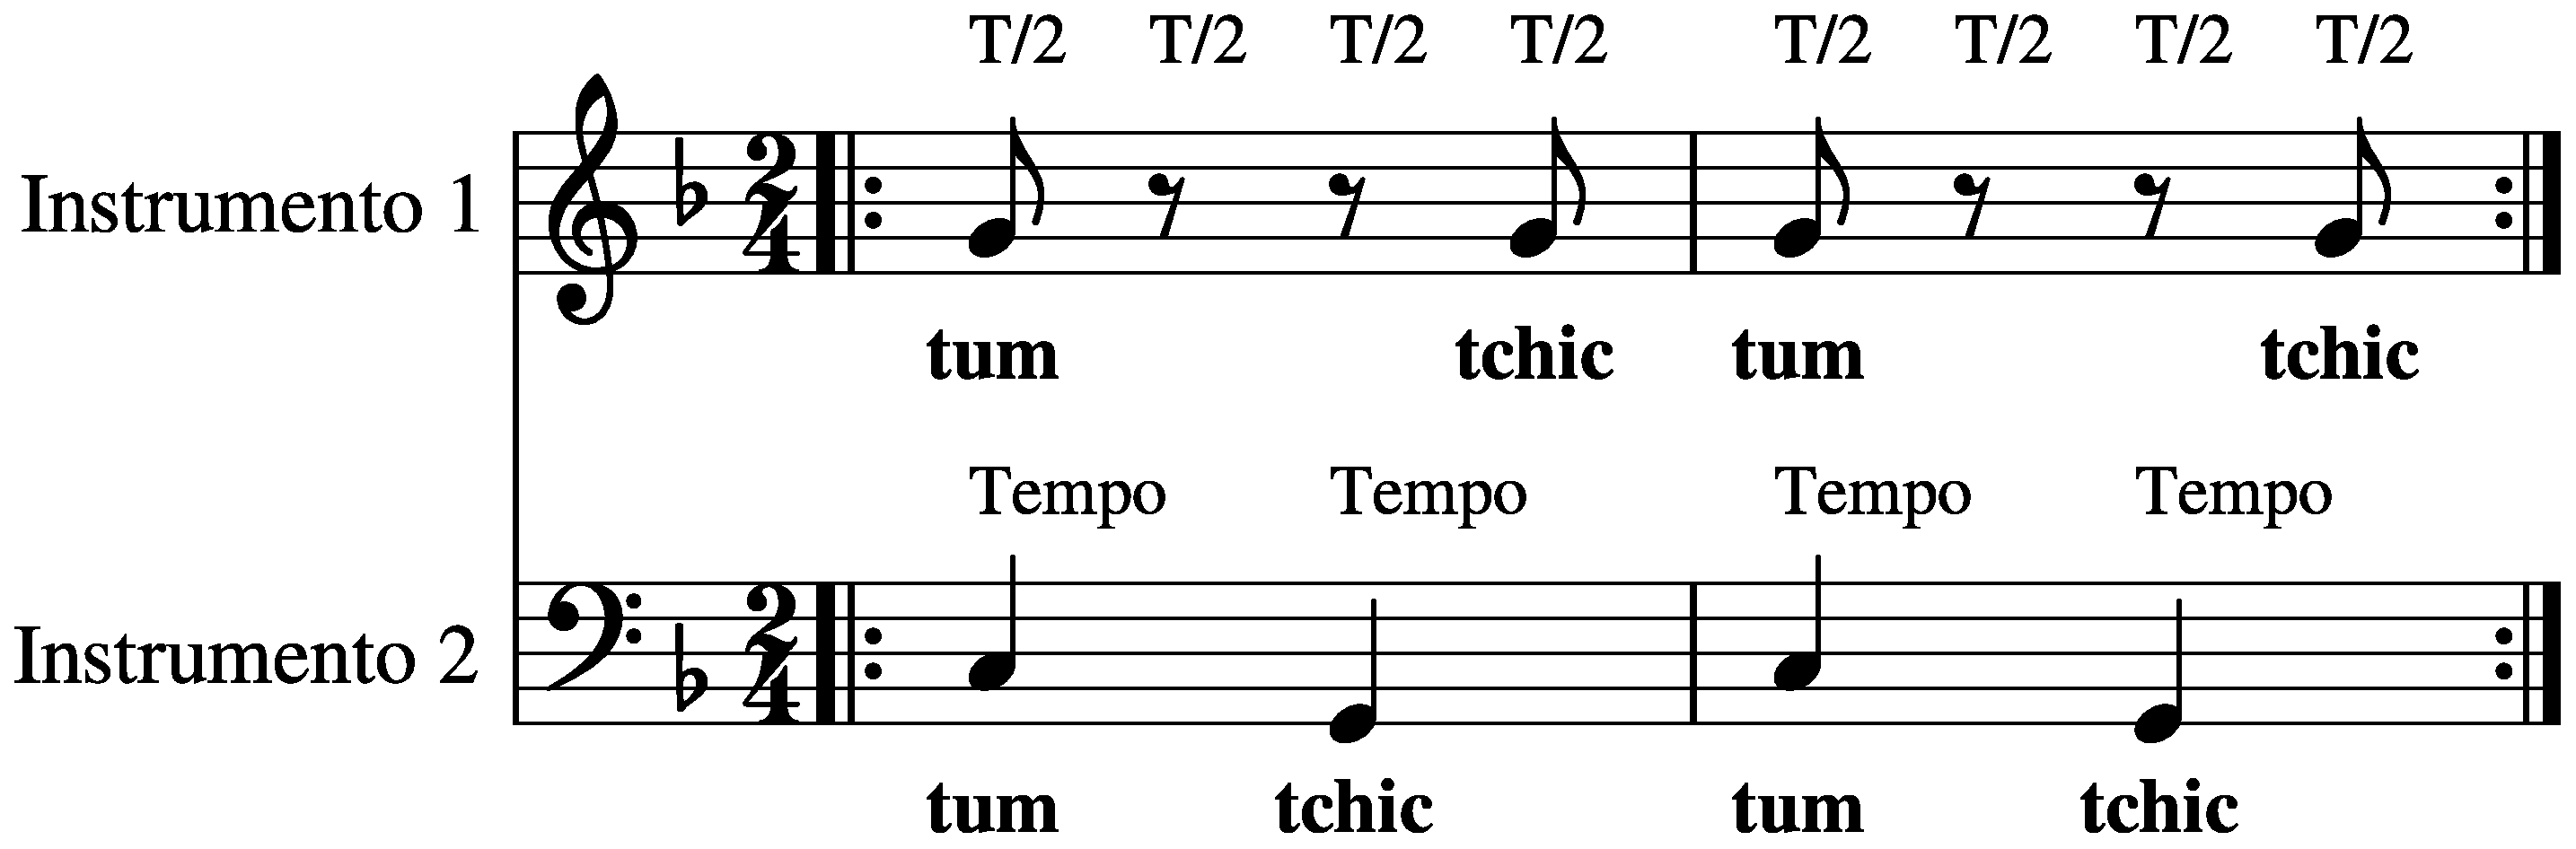
\includegraphics[width=0.8\textwidth]{chapters/cap-musicalidade-percepcion/abc-tchic-tchic-tum-1.eps}}
\begin{comment}
\begin{abc}[name=abc-tchic-tchic-tum-1,width=0.75\linewidth]
X: 1 % start of header
K: C % scale: C major
M:2/4
%T: Contratempo num compasso binário
V:1 clef=treble name="Instrumento 1" sname="Inst. 1"
V:2 clef=bass   name="Instrumento 2" sname="Inst. 2"
[V:1] |: " ""T/2"G1 " ""T/2"z1 " ""T/2"z1 " ""T/2"G1 | " ""T/2"G1 " ""T/2"z1 " ""T/2"z1 " ""T/2"G1  :|
w:    tum                tchic                       tum                   tchic           
[V:2] |:  "Tempo"C,2 "Tempo"G,,2  | "Tempo"C,2 "Tempo"G,,2  :|
w:    tum       tchic              tum       tchic            
\end{abc}
\end{comment}
\caption{Padrão de repetição para gerar um sonido de onomatopeia ``tchic tchic tum''.}
\label{fig:abc-tchic-tchic-tum-1}
\end{figure}
Na qual o instrumento 1 executa dois sonidos, de modo que o primeiro contribui ao sonido 
``tum'' e o segundo sonido gera o segundo ``tchic'' do compasso; por outro lado,
o instrumento 2 executa um ritmo com um padrão
de repetição de dois sonidos ``tum'' e ``tchic'', nesse ordem;
sendo que a nota executada no tempo forte produz um sonido mais agudo que a 
executada no tempo fraco, isto é assim para poder diferenciar melhor ambos tempos.

\begin{figure}[!h]
\begin{elaboracion}{Samba: ``tchic tchic tum'' vs. métrica}
\index{Música!Ritmo vs. Fala}
Quando reconhecemos a onomatopeia ``tchic tchic tum'' no ritmo do samba, 
podemos perceber que existe uma confusão entre 
a forma que é escrita ou encaixada esta onomatopeia na partitura e como achamos que é ao escutar ela.
Pois como é visto na Figura \ref{fig:abc-tchic-tchic-tum-1}, quando escrevemos
um ritmo cíclico com um padrão de repetição na ordem ``tum tchic tchic'' (|:\Vier \Acht \Acht:|) 
para o ouvinte é mais natural pensar que se está executando um ritmo com um padrão ``tchic tchic tum'' 
(|:\Acht \Acht \Vier:|), 
devido a que quando um ser humano fala, este usa a pausa
para denotar o final de uma palavra dado um conjunto de sílabas. Assim, ao escutar o padrão ``tum tchic tchic'', 
nossa mente otimizada para detetar palavras associa o sonido que tem um silencio maior apos ser executado,
neste caso o ``tum'' (a sílaba), com a posição final do ciclo do padrão de repetição (a palavra). 

Pelo que quando um músico vê um padrão de repetição ``tum tchic tchic'' na partitura; 
um ouvinte interpretará de forma instintiva que o padrão é ``tchic tchic tum'' iniciando em ``tchic''.
Porém não devemos confundir-nos, o ``tum'' é executado no tempo 1 do compasso.
\end{elaboracion}
\label{fig:RitmoVsFala}
\end{figure}

\subsection{Percepção do: tum~tum}

Analisando o fragmento de partitura da Figura \ref{fig:abc-caquarela} 
e tentando escutar os compassos 
para audivelmente isolar o instrumento ``D. Bass'',
podemos perceber que este gera um sonido 
com um \hyperref[sec:pos:Altura]{\textbf{tom}} muito grave, 
identificável com a onomatopeia ``tum tum'' e com uma duração de dois tempos.
No samba este ritmo é facilmente reconhecível na maioria das musicas 
e pode servi-nos de referencia quando dançamos ou quando simplesmente queremos achar o pulso.
Este instrumento é descrito isoladamente na Figura \ref{fig:abc-tum-tum-1},
na qual podemos apreciar que o compositor achou interessante diferenciar 
o tom do som que gerava o instrumento em cada tempo;
neste caso, um som mais agudo para o tempo forte e um mais grave para o tempo fraco;
porém esta diferença não é uma regra, pelo que se estamos procurando achar o tempo forte da música,
o melhor é simplesmente tentar perceber qual está sendo tocado com maior \hyperref[sec:pos:Intensidade]{\textbf{intensidade}}.
\begin{figure}[ht]
\centering
\href{https://drive.google.com/file/d/1uVEoBXD-itWcbqlr6CRrkShvS-ivBz7K/view?usp=sharing}{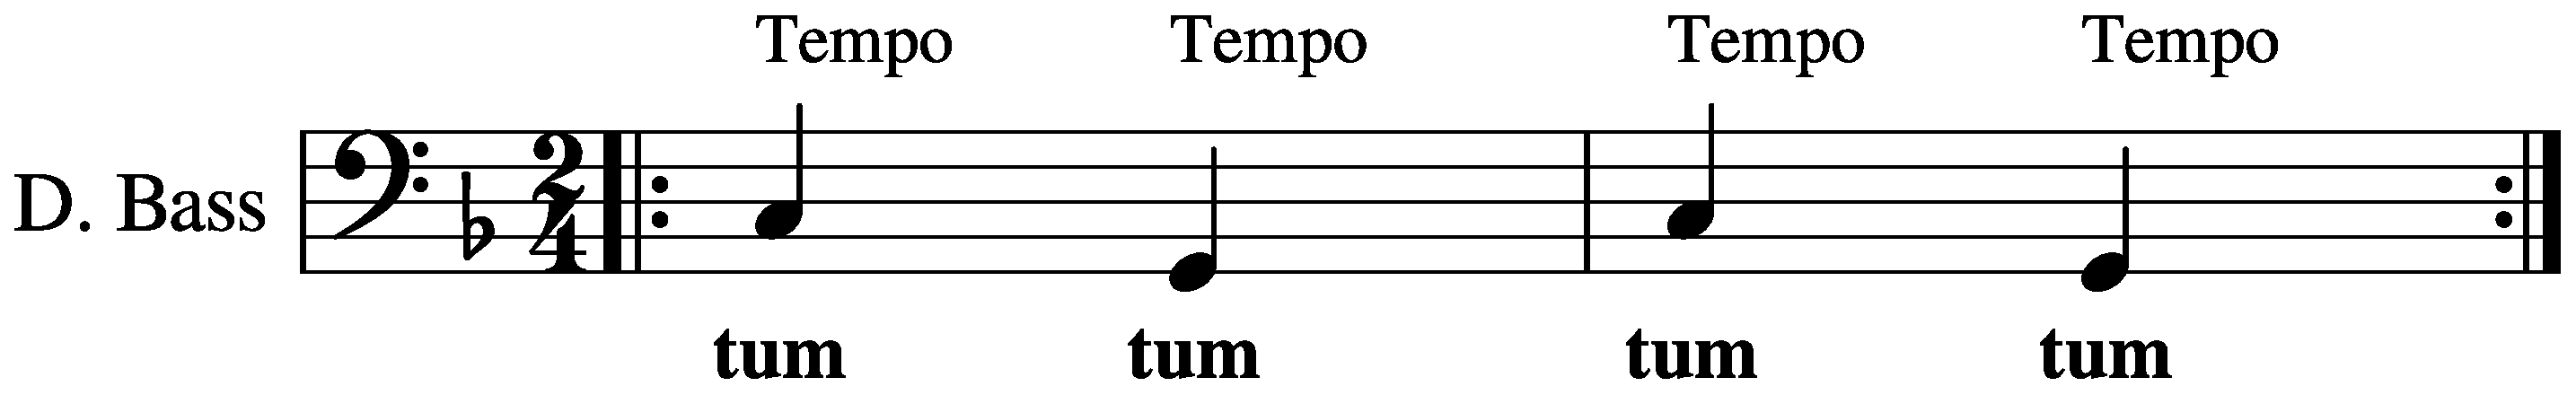
\includegraphics[width=0.9\textwidth]{chapters/cap-musicalidade-percepcion/abc-tum-tum-1.eps}}
\begin{comment}
\begin{abc}[name=abc-tum-tum-1,width=0.65\linewidth]
X: 1 % start of header
K: C % scale: C major
M:2/4
%T: Contratempo num compasso binário
V:1 clef=bass   name="D. Bass" sname="D. Bass"      
[V:1] |: "Tempo"C,2 "Tempo"G,,2  | "Tempo"C,2 "Tempo"G,,2  :|
w:    tum       tum         tum       tum            
\end{abc}
\end{comment}
\caption{Padrão de repetição para gerar um sonido de onomatopeia ``tum tum''.}
\label{fig:abc-tum-tum-1}
\end{figure}

